\section{Modelos de Memoria}

\begin{frame}{UMA vs. NUMA}
  \begin{table}
    \centering
    \begin{tabular}{@{}L{0.3\textwidth}L{0.28\textwidth}L{0.28\textwidth}@{}}
      \toprule
      & \textbf{UMA} & \textbf{NUMA} \\
      \midrule
      Memoria & Espacio compartido uniforme & Bancos locales por CPU \\
      Latencia & Constante & Depende de la distancia \\
      Escalabilidad & Limitada por bus & Alta con interconexiones rápidas \\
      C & Acceso plano; posible afinidad opcional & Requiere pinning para evitar saltos remotos \\
      Python & Copia de datos en procesos & Multiprocessing puede aislar procesos por nodo \\
      \bottomrule
    \end{tabular}
  \end{table}
\end{frame}

\begin{frame}{Implicaciones prácticas}
  \begin{itemize}
    \item Pthreads y OpenMP comparten memoria: sincronización y coherencia de caché son críticas.
    \item Multiprocessing aísla memoria y evita condiciones de carrera, pero agrega sobrecarga por serialización IPC.
    \item NumPy y BLAS liberan el GIL y usan hilos nativos, aprovechando memoria compartida de forma eficiente.
  \end{itemize}
\end{frame}

\begin{frame}{Mapa visual}
  \begin{figure}
    \centering
    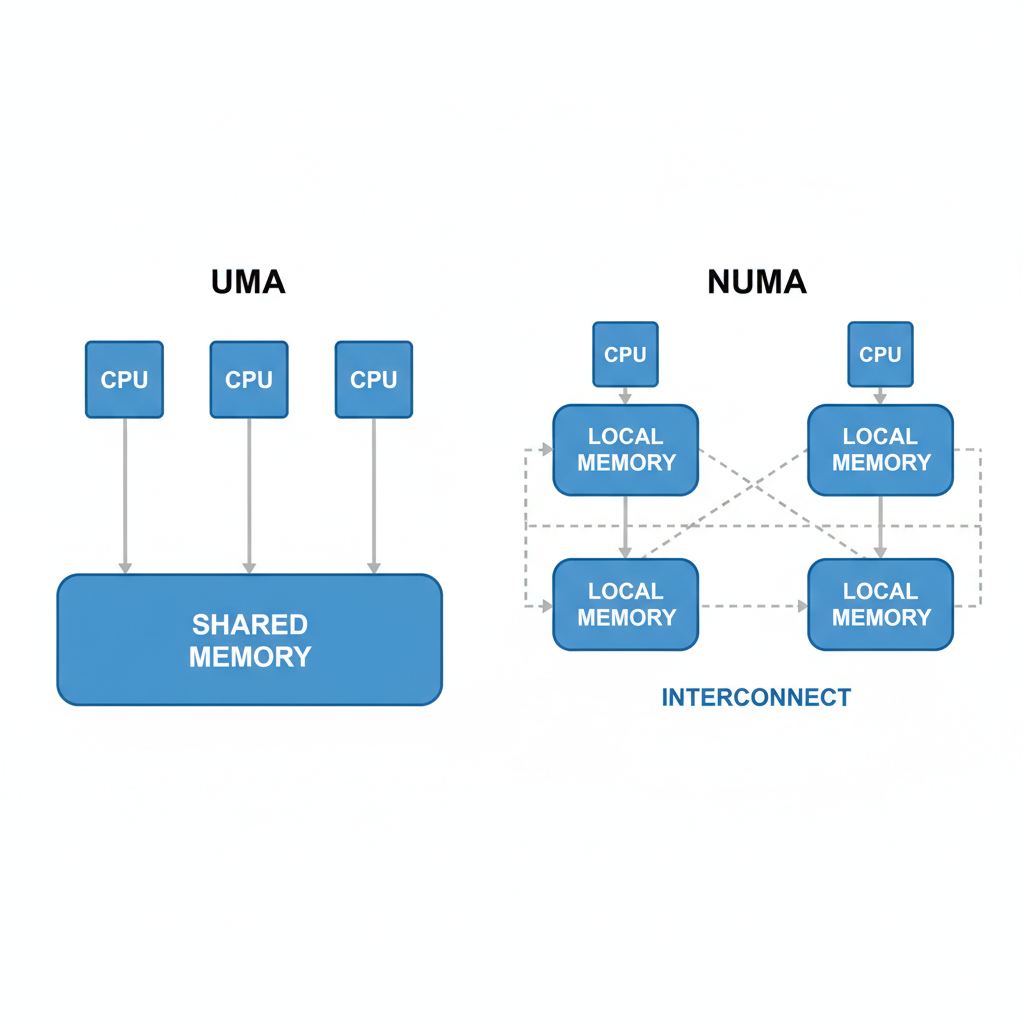
\includegraphics[height=0.6\textheight]{img/03-uma-vs-numa.png}
    \caption{Arquitecturas de memoria UMA vs. NUMA.}
  \end{figure}
\end{frame}
